\documentclass[conference]{IEEEtran}
\IEEEoverridecommandlockouts
% The preceding line is only needed to identify funding in the first footnote. If that is unneeded, please comment it out.
\usepackage{graphicx}
\usepackage{textcomp}
\usepackage{xcolor}
\def\BibTeX{{\rm B\kern-.05em{\sc i\kern-.025em b}\kern-.08em
    T\kern-.1667em\lower.7ex\hbox{E}\kern-.125emX}}
\begin{document}

\title{Neural Networks at the Edge}

\author{\IEEEauthorblockN{Deboleena Roy}
\IEEEauthorblockA{
\textit{Purdue University}\\
West Lafayette, IN \\
roy77@purdue.edu}
\and
\IEEEauthorblockN{Gopalakrishnan Srinivasan}
\IEEEauthorblockA{
\textit{Purdue University}\\
West Lafayette, IN \\
srinivg@purdue.edu}
\and
\IEEEauthorblockN{Priyadarshini Panda}
\IEEEauthorblockA{
\textit{Purdue University}\\
West Lafayette, IN \\
srinivg@purdue.edu}
\and
\IEEEauthorblockN{Richard Tomsett}
\IEEEauthorblockA{
\textit{IBM Research}\\
Hursley, UK \\
rtomsett@uk.ibm.com}
\and
\IEEEauthorblockN{Nirmit Desai}
\IEEEauthorblockA{
\textit{IBM Research}\\
Yorktown Heights, USA \\
nirmit.desai@us.ibm.com}
\and
\IEEEauthorblockN{Raghu Ganti}
\IEEEauthorblockA{
\textit{IBM Research}\\
Yorktown Heights, USA \\
rganti@us.ibm.com}
\and
\IEEEauthorblockN{Kaushik Roy}
\IEEEauthorblockA{
\textit{Purdue University}\\
West Lafayette, IN \\
kaushik@purdue.edu}
}

\maketitle
\begin{abstract}
As neural networks gain importance with several successful applications of them, this paper raises the question of how they can be applied in the context
of coalition operations. A key challenge in military coalition operations is that of energy and severe bandwidth constraints. We address this challenge by
exploring the use of Deep Neural Networks (DNNs) and splitting them across multiple edge nodes. Further, we explore the idea of using spiking neural networks
that can lower the energy consumption significantly. Preliminary results show that both these approaches can have significant impact on coalition operations.
\end{abstract}

\section{Introduction}
\label{sec:intro}
In coalition operations, mission commanders face the challenge of gaining adequate situational understanding to support decision making. In such operations, analytic and computational resources may be spread across different units. The resources may be limited in terms of compute power and energy usage. Communication between services is challenging, as networks are formed dynamically and will be both noisy and severely bandwidth-constrained. Analytic tools must therefore be implemented around these constraints, while still providing useful information to analysts and mission commanders.

Deep neural networks (DNNs) have emerged as a powerful tool for a broad variety of analytical tasks including classification, object recognition, anomaly detection, and time-series prediction~\cite{Goodfellow:2016}. As the current state-of-the-art tool in these areas, their deployment to aid coalition situational understanding is inevitable. The above-mentioned constraints on computation and energy use at edge devices in a coalition network will severely limit the capabilities of edge-deployed DNNs, which tend to perform better with increasing depth and thus increasing resource requirements. However, sending data back to the cloud for processing will usually not be possible due to network transfer limitations, so running the DNNs at the edge is still preferable.

We propose a new approach to running DNNs on coalition networks that is designed both to be compatible with the various implementation constraints and to allow appropriately deep networks for good task-performance. We build on ideas developed by Panda et al., who propose executing a subset of a full DNN's layers until adequate confidence is reached, rather than passing the input data through every network layer~\cite{panda2016conditional, panda2017energy}. This approach can reduce computation and energy consumption without reducing task performance. We propose extending this idea to evaluate different DNN layers on different edge devices depending on their availability and computational capabilities.

In the next section, we outline the motivating scenario behind this proposal and describe at a high level how DNN evaluation could be split across edge devices. We provide a detailed account of the splitting and evaluation methods in section \ref{sec:conditional}. These ideas are then extended to the case of spiking neural networks in section \ref{sec:spiking}, as these offer a promising way to further reduce the energy consumption and data transfer requirements of the proposed paradigm. Finally we provide some discussion of the approach, raise potential implementation issues, and propose avenues for further research.
\section{Scenario and Problem Statement}
\label{sec:scenario}
Our research is motivated by the need to enable situational understanding in coalition military operations. Militaries are increasingly using technology to help achieve this goal, deploying a variety of intelligent sensors for collecting and analyzing data. This has led to the development of the “Internet of Battlefield Things” (IoBT) concept to describe future military operations. In the IoBT, the “things” (e.g. sensors, vehicles, robots, wearable devices) will be augmented with various levels of intelligence, and will communicate with each other to coordinate their operations, as well as with their human users to facilitate sensemaking~\cite{Kott:2016, Suri:2016}.

The battlefield setting presents a number of barriers to achieving this vision. Information flow constraints are a major challenge: devices will be distributed and move around over a wide geographical area, often in regions with poor or no communications infrastructure. Communications will need to be wireless -- for example via satellite link or cellular networks -- but these methods suffer from high latency, as well as being potentially costly. The current popular model of providing devices with intelligent behaviours by transferring their data to back-end cloud services for processing will not be possible. Devices will therefore require local data processing and intelligence capabilities~\cite{Verma:2017}.

However, edge devices are also locally resource-constrained in terms of compute capability and energy consumption. A particular device may be serving many different requests from different users, and with limited local compute capacity could quickly become overloaded. If battery powered, the device will also need to minimize its energy consumption by reducing the number of computations it performs, while still remaining useful to the coalition.

In this paper, we explore a method that addresses these issues in the case of edge devices running deep neural networks (DNNs). DNNs have proven extremely effective for a variety of machine learning tasks including data classification, time-series prediction, anomaly detection, and speech/language processing~\cite{LeCun:2015, Goodfellow:2016}. The power of DNNs comes from their capacity to learn rich, hierarchical representations from data~\cite{Bengio:2013}. The term “deep” refers to the number of layers used to learn these representations. For complex data such as video, audio, or images, deeper models with more layers tend to perform better than shallower models~\cite{Szegedy:2015}. However, as the depth of the model increases, so do the computational requirements, meaning that DNNs may not be practical for deployment on computationally-limited or energy-constrained edge devices.

We propose exploiting the hierarchical nature of the learned representations in a DNN to adaptively distribute the computation over the edge devices in the coalition network. Our method builds on work by Panda et al., which showed how the energy consumption of DNN computation could be reduced by considering the output of one network layer at a time, and only computing the output of the next layer if the confidence of the output based on the current layer was low~\cite{Panda:2016}. This minimizes computational requirements by cutting out unnecessary processing by deeper layers for “easier” inputs. Our approach proposes distributing the computation of different layers between different devices on the network. Using this scheme, the processing requirements on the first device are minimised, and if further processing by deeper layers is required, another device can be called on to do this if the first device needs to reduce its computational load. This process can be chained, potentially involving as many devices as there are network layers.

\begin{figure}[ht]
\centering
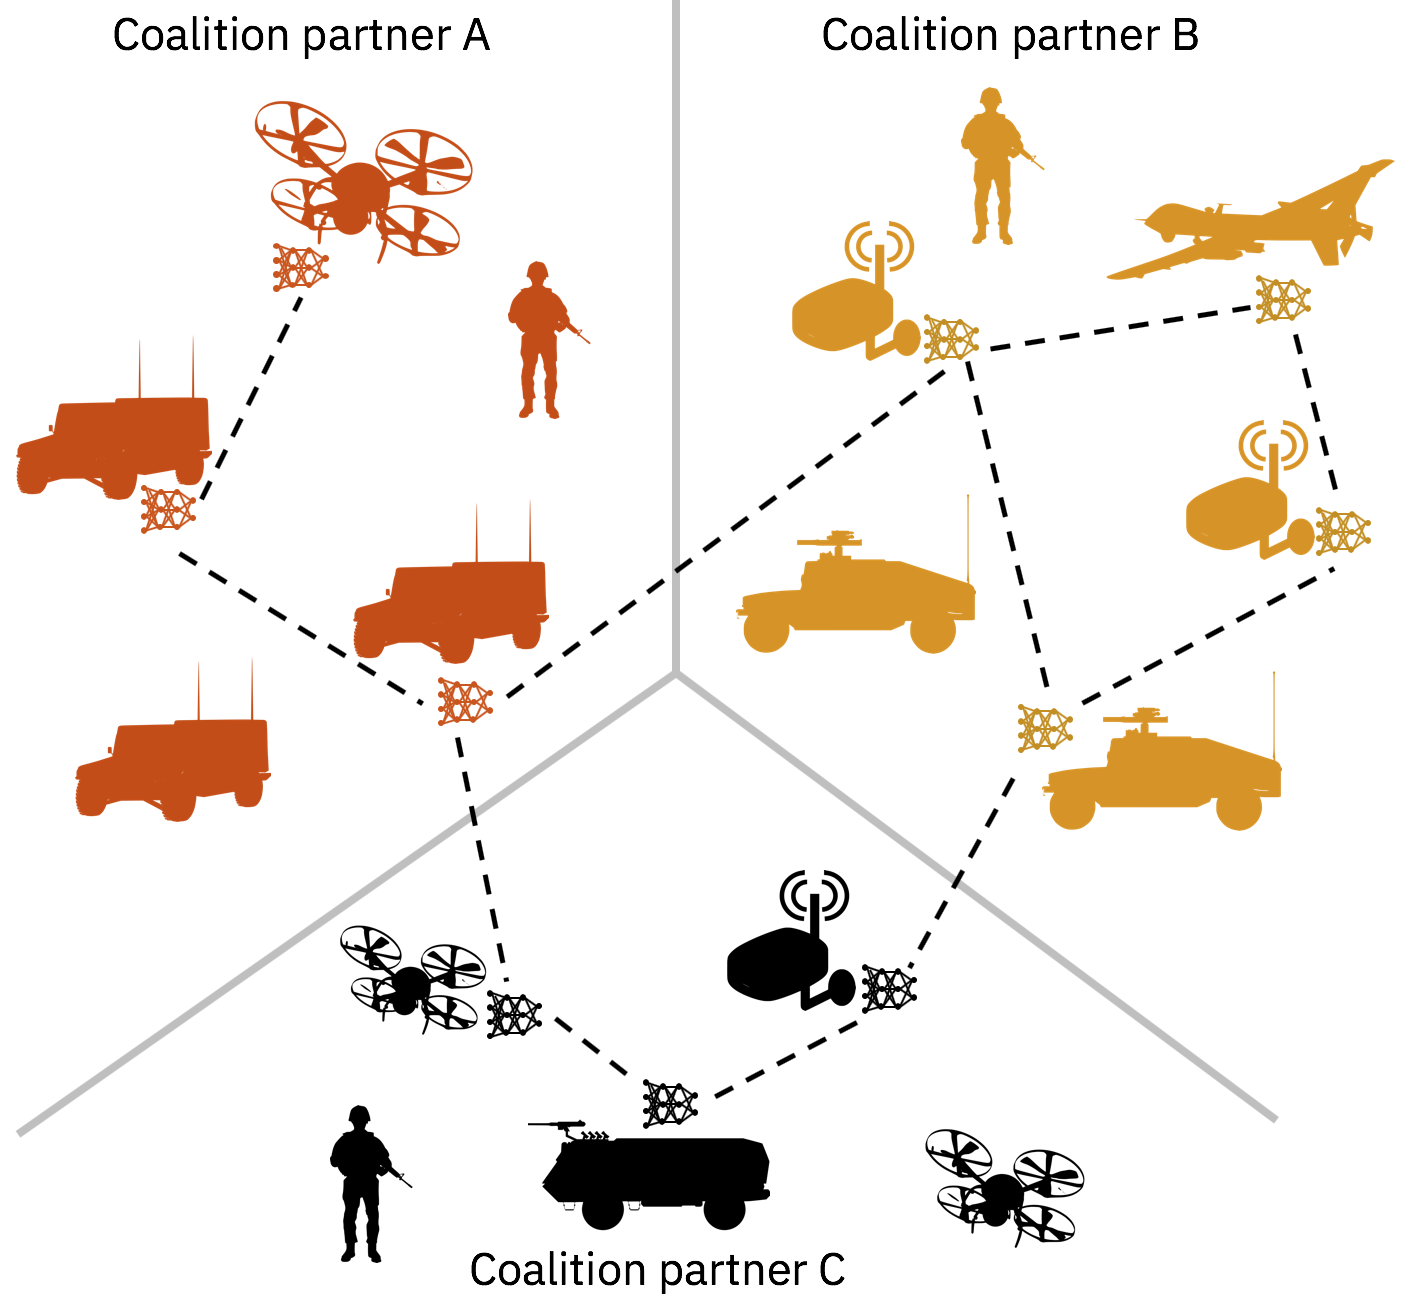
\includegraphics[width=0.49\textwidth]{fig1.png}
\caption{Conceptual illustration of the IoBT, and the proposed distribution method for DNNs. In this example, three coalition partners are collaborating. Each partner has deployed intelligent devices to the battlefield. Several of these devices have the same DNN deployed on them, and so can distribute computation between them layer by layer.}
\label{fig:coalition}
\end{figure}
\section{Conditional Deep Neural Networks}
\label{sec:conditional}
%Explain the conditional, pointing to the existing work. https://arxiv.org/pdf/1509.08971.pdf

%Identify any issues/drawbacks with this approach. How much information/confidence can be derived?
%Will interpretability be an issue and how much extra information be gathered from the task being partially completed?

Conventional deep neural networks (DNNs) have scaled greatly in depth, from 8 layers in AlexNet \cite{krizhevsky2012imagenet} to 1000 layers in ResNet-1001 \cite{he2016identity}. With the increase in size, the cost of implementing these very deep networks have increased as well. In order to determine the classification result, the input is processed through all the layers of the DNN, thereby consuming a lot of time and effort. However, in real world, not all inputs are made equal, and one can ideally design algorithms whose complexity is proportional to the difficulty of the input \cite{venkataramani2015scalable}. Such a design can provide both energy efficiency and speed up. Conditional Deep Learning \cite{panda2017energy, panda2016conditional} is a technique of augmenting deep neural networks with linear classifiers at the output of intermediate layers, that gives the user the control to conditionally activate the deeper layers of the network. 

In a Conditional Deep Learning network (CDLN), there are conditional exits added to the network after every few layers. As shown in Fig. \ref{fig:CDL-1}, when an input is presented to the network, the first linear classifier outputs the classification probability of the image. If the classifier has a strong confidence, that is the maximum output is beyond a threshold, then the network assigns the corresponding label to the input. If the confidence value is lower than threshold, then the next layers are activated and we move to the next classifier. These linear classifiers can be trained in tandem while training the whole network, or can be trained separately after the network is fully trained. 

\begin{figure}[h]
\centering
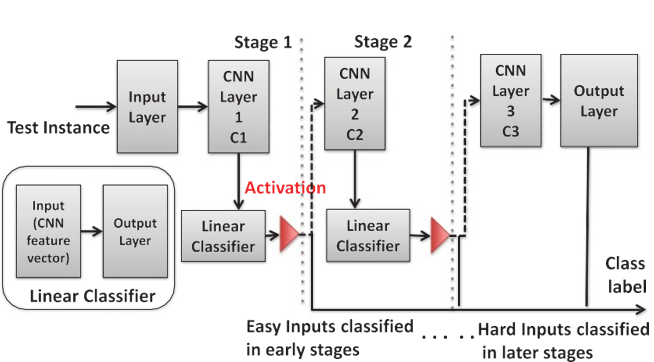
\includegraphics[width=0.45\textwidth]{CDL_1.png}
\caption{Conditional Deep Learning Network (CDLN) with linear classifiers added at the convolutional layers whose output is monitored to decide if classification can be terminated at current stage or not.} \label{fig:CDL-1}
\end{figure}

CDLN \cite{panda2017energy} offers $1.84\times$ improvement in energy in comparison to traditional implementation for MNIST on LeNet-5 \cite{lecun1998gradient}, which increases to $4.96\times$ for TinyImagenet implemented on ResNet-50 \cite{he2016deep}. Along with energy improvements, CDLN also offers significant improvement in inference time. As the whole network doesn't need to be activated for all the examples, average inference time per example reduces. It is reported in \cite{panda2017energy}, that CDLN implementation speed up the inference by $4.24\times$ for MNIST and $1.71\times$ for TinyImagenet. 

For a resource-constrained environment, CDLN offers an unique solution, that has both energy and timing improvements. In \cite{parsa2017staged}, conditional deep learning is used to implement staged inference for fast real time applications. For applications involving distributed intelligence, CDLN offers a framework that can be split up and deployed across edge and cloud. A low power system with low compute capabilities can be used to execute the the initial layers of the network. The linear classifier at the end of the first stage can provide us with some information regarding the input with a certain degree of confidence. In situations where the confidence of the edge is low, the data can be transmitted to the cloud to be processed by the remaining layers of the network. 













\section{Spiking extensions}
\label{sec:spiking}
The state-of-the-art DNNs are compute-intensive since they operate on real-valued inputs, leading to higher energy consumption in resource-constrained edge devices with limited power budget. In this regard, Spiking Neural Networks (SNNs) offer a promising solution for enabling energy-efficient neuromorphic computing in the edge nodes. SNNs process and encode input information temporally using sparse spiking events. The intrinsic sparse event-driven computing capability of SNNs can be exploited to achieve higher energy efficiency in hardware implementations as shown in \cite{sengupta2019going, blouw2018benchmarking}. The inherent computational efficiency of SNNs can be attributed to the fact that every layer of an SNN needs to compute the weighted sum of the input spikes with the synaptic weights only in the event of a spike fired by the corresponding input neurons. Furthermore, computing the weighted input sum requires only adders since the inputs are encoded as spikes that are represented by logic states \{0, 1\}. On the contrary, DNNs require multipliers, which consume at least an order of magnitude higher energy than adders, for computing the weighted input sum since they operate on real-valued inputs.

SNNs are naturally suited for splitting and conditional evaluation among different edge nodes because of the following two-fold reasons. First, they improve the energy efficiency per edge node due to inherent sparse event-driven processing capability as mentioned in the previous paragraph. Furthermore, researchers in \cite{sengupta2019going} demonstrated that sparsity in spiking activity increases substantially across successive layers of a deep SNN. Hence, energy efficiency would be further enhanced for edge nodes evaluating the deeper layers of an SNN. Second, SNNs minimize the communication overhead since only the sparse spiking events need to be transmitted between the edge nodes. Despite the computational and communication energy benefits offered by SNNs, the challenges relating to the training complexity of deep SNNs need to be addressed to champion their wide-spread adoption for real-world applications. Needless to say that efficient training strategies for deep SNNs is a current area of active research interest.

The training methodologies for deep SNNs can be broadly divided into the following three categories:
\begin{enumerate}
    \item DNN-to-SNN conversion
    \item Spiking backpropagation
    \item Spike Timing Dependent Plasticity (STDP)
\end{enumerate}
In the DNN-to-SNN conversion approaches, a DNN is trained using artificial rate-based neurons with state-of-the-art backpropagation algorithms and then mapped to deep SNN by substituting the artificial neurons with appropriate spiking neuron models and suitably normalizing the trained weights \cite{cao2015spiking, hunsberger2015spiking, diehl2015fast, rueckauer2017conversion, sengupta2019going}. The conversion approaches have been shown to be almost loss-less for deep VGG and ResNet architectures for complex vision datasets. However, the conversion approaches typically incur larger inference latency for achieving the best accuracy. The inference latency can be minimized by using the proposed splitting and conditional evaluation approach. Alternatively, the inference latency can also be optimized by training deep SNNs using spike-based backpropagation algorithms that use differentiable approximations for the spiking neurons for error backpropagation \cite{lee2016training, panda2016unsupervised, wu2018spatio, lee2018training, jin2018hybrid, shrestha2018slayer, neftci2019surrogate}. However, the SNN backpropagation algorithms incur longer training time compared to the DNN-to-SNN conversion approaches while offering the potential to lower the inference latency under iso-accuracy conditions. The final approach uses bio-plausible layer-wise STDP-based local learning rules to self-learn hierarchical input representations in an unsupervised manner \cite{diehl2015unsupervised, masquelier2007unsupervised, srinivasan2018stdp, tavanaei2018training, kheradpisheh2018stdp, ferre2018unsupervised, thiele2018event, lee2018deep, mozafari2018combining}. The STDP-based training rules are appealing for edge devices since they can be implemented with minimal hardware overhead compared to backpropagation algorithms. However, the STDP-trained SNNs proposed until now are only few (two to three) layers deep. It is not yet clear if the STDP-based learning rules are effective for the later layers of deeper SNNs.

Finally, we note that binary SNNs, which use binary weights \{$-$1, 1\} and spiking activations \{0, 1\}, can be used to achieve both memory- and energy-efficiency in the edge nodes. Binary DNNs, on the contrary, use either \{$-$1, 1\} \cite{courbariaux2015binaryconnect} or \{$-\alpha$, $\alpha$\} \cite{rastegari2016xnor} where $\alpha$ is a layer-specific scaling factor for the weights and binary neuronal activations \{$-$1, 1\}. Hence, every layer of binary DNNs still needs to compute the weighted input sum (XNOR operation followed by population count) for all the input neurons and transmit the binary activations of all the output neurons. However, binary SNNs need to compute the weighted input sum (AND operation followed by population count) only in the event of a spike fired by the corresponding input neurons and transmit only the sparse spiking activations of the output neurons, leading to potentially much higher energy efficiency. Binary SNNs can be trained off-line using binarization algorithms proposed for DNNs that require the full-precision weights to be stored during training \cite{courbariaux2015binaryconnect, rastegari2016xnor, hubara2017quantized}. Alternatively, binary SNNs can also be trained on-chip using stochastic-STDP based learning rules that achieves plasticity by probabilistically switching the binary weights based on spike-timing \cite{suri2013bio, querlioz2015bioinspired, srinivasan2016magnetic, srinivasan2019restocnet}. Stochastic-STDP trained binary SNNs, which eliminate the need for storing the full-precision weights, are attractive for memory- and energy-efficient learning as well as inference in the edge nodes.

\section{Related Work}
\label{sec:related}
Prior works closely related to CDLNs and SNNs have been extensively
referenced in the above sections. Previous works on addressing the
broader resource challenges for DNNs fall into three main categories:
(a) compressing the DNN models to reduce their footprint, (b)
branching and early-exit to cut down the cost of inference, and (c)
algorithmic optimizations in the compute-intensive parts of the
training and inference steps.  In the following, we constrast the
proposed ideas of this paper with these works.

\noindent{Model compression} Network compression schemes aim to reduce
the the total number of model parameters of a deep network and thus
reduce the resources required to perform inference. A pruning approach
to remove network connections having small contributions is one of the
common techniques \cite{Han-DeepCC-2015}. SqueezeNet achieves
AlexNet-level accuracy on ImageNet with 50x fewer parameters and
models smaller than 0.5MB using downsampling techniques
\cite{SqueezeNet-2016}. Whereas compression has benefits in terms of
resource consumption, thisa paper goes further in distributing network
layers across devices with CDLN-based early exits on top of SNN-based
architectures.

\noindent{Early exit} With the purpose of regularizing the main
network, Szegedy et al. \cite{Szegedy-regluar-2015} introduced the
concept of adding softmax branches in the middle layers of their
inception module. BranchyNet \cite{BranchyNet-2016} extends CDLN by
jointly training early exit branch networks. Recently, thin vertical
sub-networks, as opposed to shallow sub-networks as achieved with
CDLN, are proposed to enable ``anytime'' prediction according to
resource availability \cite{Lee-Anytime-2018}.  We leverage the key
ideas of CDLN in this paper and introduce horizontal slicing across
multiple edge nodes and leverage SNNs to reduce footprint and resource
requirements.

\noindent{Algorithmic optimizations} FFTs have been widely used for
efficient convolution on large convolutional filters
\cite{Mathieu-Fast-2014}. Building on this, faster algorithms
specifically for smaller 3x3 convolutional filters (which are used
extensively in VGGNet and ResNet), and smaller batch sizes
specifically important in an edge scenario have been proposed
\cite{Lavin-Fast-2016}. These improvements are relevant and orthogonal
to the CDLN paradigm with SNN-based architectures.


\section{Discussion}
The proposed distribution method for DNN inference poses a number of challenges. A crucial consideration is the balance between computation and data transmission. Military coalition operations will likely be limited in both respects, but the optimal balance for deciding what to compute locally versus what to send to other nodes will vary over the coalition network and depend on the following factors:

\begin{itemize}
    \item Local compute availability: the computational resources, and how available those resources are given any other local computing tasks;
    \item Local energy availability: what level of computation and data transmission the device's energy supply supports, and how long this will last given the projected device usage; and
    \item Network transmission capability: the speed and reliability of the network to transmit data between devices.
\end{itemize}

As discussed above, CDLNs can reduce both local computation and local energy consumption over conventional DNNs. The proposed distribution method can further reduce local computation by offloading the processing of higher CDLN layers either to the cloud or to other edge devices. However, this requires the device to transmit data over a potentially slow and unreliable network. A balance must be reached between the cost (both in terms of energy and computation) of running the network locally, and the cost of sending data to other nodes.

A naive implementation of the distributed evaluation method might transmit the full output of a CDLN layer, which for large networks dealing with high dimensional inputs could amount to several hundred kilobytes or more. This could prove unfeasible in a coalition network. A simple approach for reducing data transfer in conventional (non-spiking) CDLN implementations is simply to reduce the bit-depth of the network. This approach has been found to maintain accuracy with networks implemented using 8-bit integers, immediately quartering the required data transfer compared with standard floating point representations~\cite{jacob2018quantization}. Further data reduction methods could also be employed, such as only transmitting layer outputs larger than a certain threshold. However, as discussed in section \ref{sec:spiking}, an even more efficient method would be to implement the CDLN as an SNN and transmit binary spikes between nodes. This not only reduces data transmission requirements, but also improves the robustness of the transmission to unreliable networks: SNNs are inherently robust to stochastic variation in spike trains, meaning that they would cope well with noisy data transmission between nodes.

Another limitation of the proposed method is that it requires copies of the CDLN to be available either in the cloud or on other edge devices. This is unlikely to be the case when the coalition is rapidly formed and dynamic. This limitation may be addressed by researching how to make different DNNs interpretable to each other, such that the output of a layer in one network could be interpreted appropriately by a layer in a different network. In this way, layer outputs from a CDLN could be processed by CDLNs on other devices provided that these CDLNs were \textit{similar enough} to the originating CDLN. The concept of inter-model interpretability has previously been formalized by Dhurandar et al. under the framework of \(\delta\)-interpretability \cite{deltaInterpretability,TIPInterpretability}, but research remains to be done on how to achieve it in practice.

\section{Conlusions}
\label{sec:conclusions}

\section*{Acknowledgements}
This research was sponsored by the U.S. Army Research Laboratory and the U.K. Ministry of Defence under Agree- ment Number W911NF-16-3-0001. The views and conclusions contained in this document are those of the authors and should not be interpreted as representing the official policies, either expressed or implied, of the U.S. Army Research Laboratory, the U.S. Government, the U.K. Ministry of Defence or the U.K. Government. The U.S. and U.K. Governments are au- thorized to reproduce and distribute reprints for Government purposes notwithstanding any copyright notation hereon.


\bibliographystyle{IEEEtran}
\bibliography{references}

\end{document}
